\section{Extras}

\begin{frame}{Propensity Score Issues}
 \begin{itemize}
  \item Unmeasured confounders
  \item Choice of pretreatment covariates in the propensity score model
  \item Different models and methods may lead to different conclusions
 \end{itemize}

\end{frame}

\begin{frame}{Joint Modelling (JM)}
 \begin{itemize}
  \item Assume ignorable MAR  missing data mechanism
  \item Missing data imputed by sampling from a user specified distribution
  \item A lot of theory developed for Normal, not much else
  \begin{itemize}
   \item Normal imputation has been shown to perform well, even under non normality \cite{Demirtas2008}
  \end{itemize}
\item Idea: pull imputations by missing data row pattern
 \end{itemize}

\end{frame}

\begin{frame}{JM pseudocode}
 \begin{figure}[h!]
  \centering
    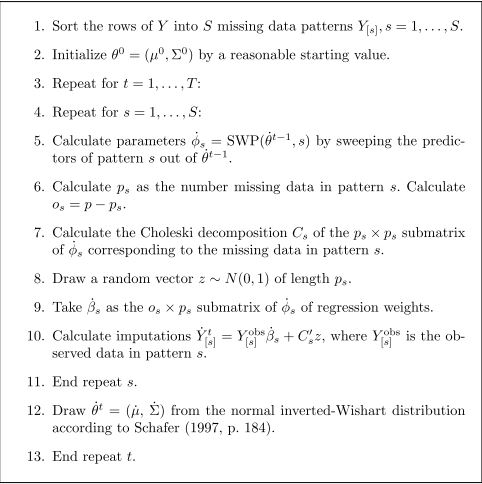
\includegraphics[width=0.6\textwidth]{jm_algo}
 % \caption{Normal JM imputation pseudocode}
\label{fig:jmexample}
\end{figure}
%do I want to include the amelia algo?
\end{frame}

\begin{frame}{JM Pros and Cons}
Pros
 \begin{itemize}
  \item Fast
  \item Easy to derive posteriors with common distributions
 \end{itemize}

 Cons
 \begin{itemize}
  \item Inflexible
  \item Limited to known distributions
  \item How to deal with mixed categorical and continuous missing data
 \item Poor with derived variables
 \item Can give impossible combinations
 \end{itemize}

\end{frame}

\begin{frame}{The Stack Method}
 \begin{itemize}
  \item Rubin's Rules work well, but not always
  \begin{itemize}
   \item Ex: partitioning the MI data on an imputed variable
   \item Taking the average is not a good idea
  \end{itemize}
    \item Solution: Stack the MI datasets on top of each other to get one huge dataset
    \begin{itemize}
     \item Will get unbiased results
     \item But sample size is falsely inflated, thus cannot trust variance
    \end{itemize}
 \end{itemize}
 \begin{figure}[h!]
  \centering
    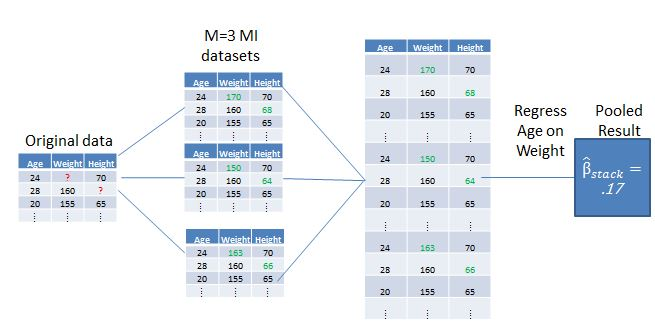
\includegraphics[width=0.6\textwidth]{stacked}
 % \caption{Normal JM imputation pseudocode}
\label{fig:stacked}
\end{figure}
\end{frame}

\begin{frame}{KM issues in the MI setting}
\begin{itemize}
\item Issue: Kaplan-Meier is not normally distributed
  \begin{itemize}
   \item Solution: Complimentary log log transformation, pool \cite{Marshall2009}
  \end{itemize}
  \item Issue: Imputations leave one KM curve much shorter than the rest
  \begin{itemize}
   \item Solution 1: Truncate all curves at the lowest time
   \item Solution 2: Extend the curves out to the longest time
   \item Solution 3: Use the stacked method
  \end{itemize}

\end{itemize}
\end{frame}

\begin{frame}{Log Rank Issues in MI setting}
\begin{itemize}
  \item Idea: Combine log rank tests from each MI dataset
  \begin{itemize}
  \item Problem: Wastes information and is unstable \cite{Marshall2009}
  \item Idea: Calculate log rank from the MI Kaplan-Meier curve
  \item Problem: Risk set and deaths no longer meaningful
  \end{itemize}
\end{itemize}
\end{frame}

\begin{frame}{Setting up the model- Issues}
\begin{itemize}
 \item Many categorical variables 
 \item Collinearity between predictors
 \item Variables with poor influx/outflux \cite{VanBuuren2012}
 \item How many iterations and imputations to draw?
\end{itemize}

\end{frame}


\begin{frame}{Validity Checks}
 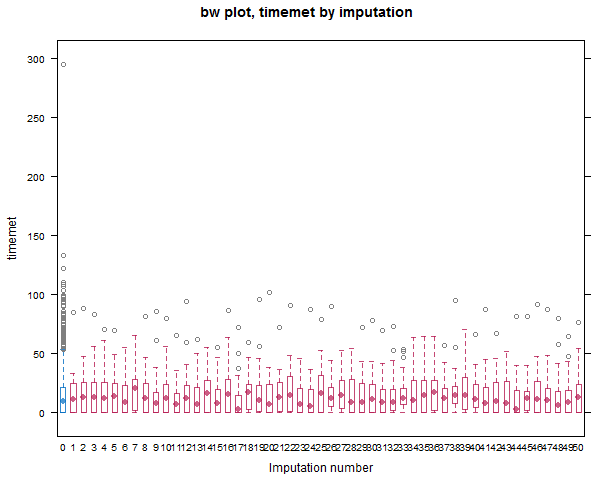
\includegraphics[width=.5\textwidth]{bw_timemet}%
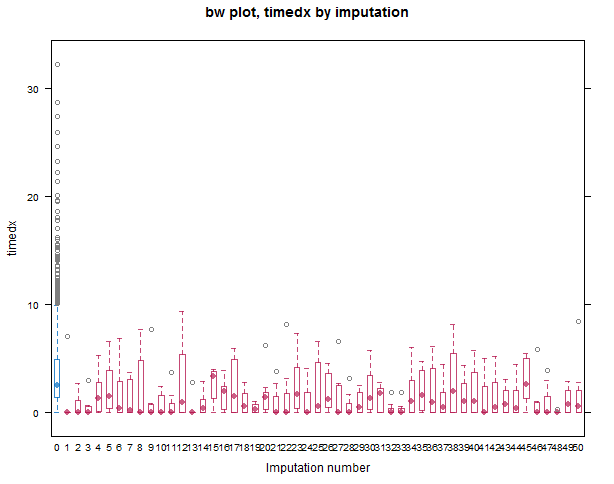
\includegraphics[width=.5\textwidth]{bw_timedx} 
\end{frame}

\begin{frame}{Tabluar Checks}
 \begin{figure}[h!]
  \centering
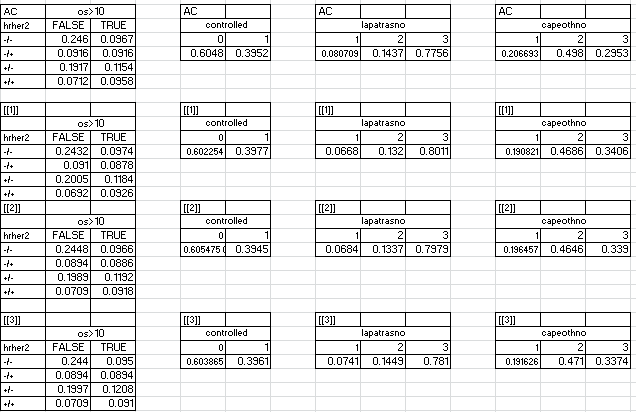
\includegraphics[width=.8\textwidth]{tabchecks} 
  \caption{Selected tabluar checks}
\label{fig:tabcheck}
\end{figure}

\end{frame}


\begin{frame}{Issues with Propensity Score in our Setting}
\begin{itemize}
 \item Problem: Theory was developed for binary treatments, we have ternary
 \begin{itemize}
  \item Solution: Run each treatment as binary, then compare groups
 \end{itemize}
\item Propensity score model specification
\begin{itemize}
 \item Solution: Boosting, subject to KS statistic minimization
\end{itemize}
\end{itemize}
 
\end{frame}

%put boosting algo here if I have time
